\section{Numeric Solution To The Diffusion Only Equation}


As a first approach to the problem, we will use an implicit scheme to find the numerical solution. This means that, in approaching the finite difference method, we will compute the spacial derivative at time step $n+1$. 
Just as in the analytic case, we define
\begin{align}
	\rho(x,t) = C(x,t) - C_b
\end{align}

Consider the one dimensional diffusion equation

\begin{align}
\frac{\partial \rho}{\partial t} &= D \frac{\partial^2 \rho}{\partial x^2}.
\label{eq:diffusion}
\end{align}

We will define $x = \delta \xi$ where $\delta$ is the width of the laminar flow sheet. 

\begin{align}
\frac{\partial \rho}{\partial t} = \frac{D}{\delta^2} \frac{\partial^2 \rho}{\partial \xi^2},\\
\frac{\partial \rho}{\partial \tau} =  D \frac{\partial^2 \rho}{\partial \xi^2},
\end{align}

where we have defined $\tau = t/\delta^2$
We will discretize the derivative as follows,

\begin{align}
\frac{\partial \rho}{\partial \tau}^{n+1, k}= \frac{C^{n+1, k}-\rho^{n, k}}{\Delta \tau},\\
\frac{\partial^2 \rho}{\partial \xi^2}^{n+1, k} = \frac{\rho^{n+1, k-1}-2\rho^{n, k}+\rho^{n+1, k+1}}{\Delta \xi^2}.
\end{align}

Replacing these approximations into equation \ref{eq:diffusion} we get

\begin{align}
    -\alpha \rho^{n+1,k-1} + ( 1 + 2\alpha ) \rho^{n+1,k} -\alpha \rho^{n+1,k+1} =  \rho^{n,k}\\
    k \in [1, ... , m-1]
    \label{eq:equations-n}
\end{align}

In particular, for a given $n$ value,  the equations for $k=1$ and $k=m-1$ (which include the border conditions) are

\begin{align}
    -\alpha \rho^{n+1,0} + ( 1 + 2\alpha ) \rho^{n+1,1} -\alpha \rho^{n+1,2} = \rho^{n,1},\\
    -\alpha \rho^{n+1,m-2} + ( 1 + 2\alpha ) \rho^{n+1,m-1} -\alpha \rho^{n+1,m} = \rho^{n,m-1}.
    \label{eq:border-equations}
\end{align}

The border conditions for our system (in discretized form) are

\begin{align}
    \rho^{n, 0} = \rho^{n, 1}, \\
    \rho^{n, m-1} = 0.
\end{align}

Therefore, equations \ref{eq:border-equations} yield

\begin{align}
    ( 1 + \alpha ) \rho^{n+1,1} -\alpha \rho^{n+1,2} = \rho^{n,1},\\
    -\alpha \rho^{n+1,m-2} + ( 1 + 2\alpha ) \rho^{n+1,m-1} = \rho^{n,m-1}.
\end{align}

We want to put these equations in matrix form. Let 

\begin{align}
    \bf{\rho^n} = \begin{bmatrix}
                    \rho^{n, 0} \\
                    \rho^{n, 1} \\
                    \vdots \\
                    \rho^{n, m-1} \\
                    \rho^{n, m} \\
                    \end{bmatrix},
\end{align}

and 

\begin{align}
\bf{\underline{A}} &= \begin{bmatrix}
           ( 1 + \alpha ) & -\alpha  &  0 & 0 &  \cdots & 0\\
             -\alpha & ( 1 + 2 \alpha ) & -\alpha & \cdots & 0 & 0\\
           \vdots  &\cdots  & \ddots & \ddots &  \ddots&  \\
            \vdots & \cdots & 0  &  -\alpha & ( 1 + 2 \alpha ) & -\alpha \\
            0 & \cdots &0  & 0 & -\alpha & ( 1 + 2 \alpha )
         \end{bmatrix}
         \label{eq:discretization-matrix}.
\end{align}

Equations \ref{eq:equations-n} can be expressed as

\begin{align}
    \bf{\underline{A}} \bf{\rho^{n+1}}  = \bf{\rho^n} .
\end{align}

Considering the initial conditions \ref{eq:initial-condition}, we get

\begin{align}
    \bf{\rho^{0,k}} = -C_b, \\
    k \in [1,..., M-1].
\end{align}

This means that the shape of $\bf{\underline{A}}$ is $M-2 \times M-2$ and the numerical solution is solved in the interval  $k \in [0,..., M]$, leaving $k=0$ and $k=M$ as the overflow terms to push the boundary conditions. Nevertheless, these terms must be included in order to get the full solution (otherwise we should start from $k=1$ and end at $k=M-1$ and not include the border conditions in the plot of our numeric result).

Now we are ready to start iterating this matrix equation to get the time evolution.

We will use the parameters $\xi = x/\delta$ and $\tau = t/\delta^2$ as the parameters of the equation. The comparison between numeric and analytic results is shown in figure ]ref{diffusion-comparison}.

\begin{figure}[htbp]
\centering
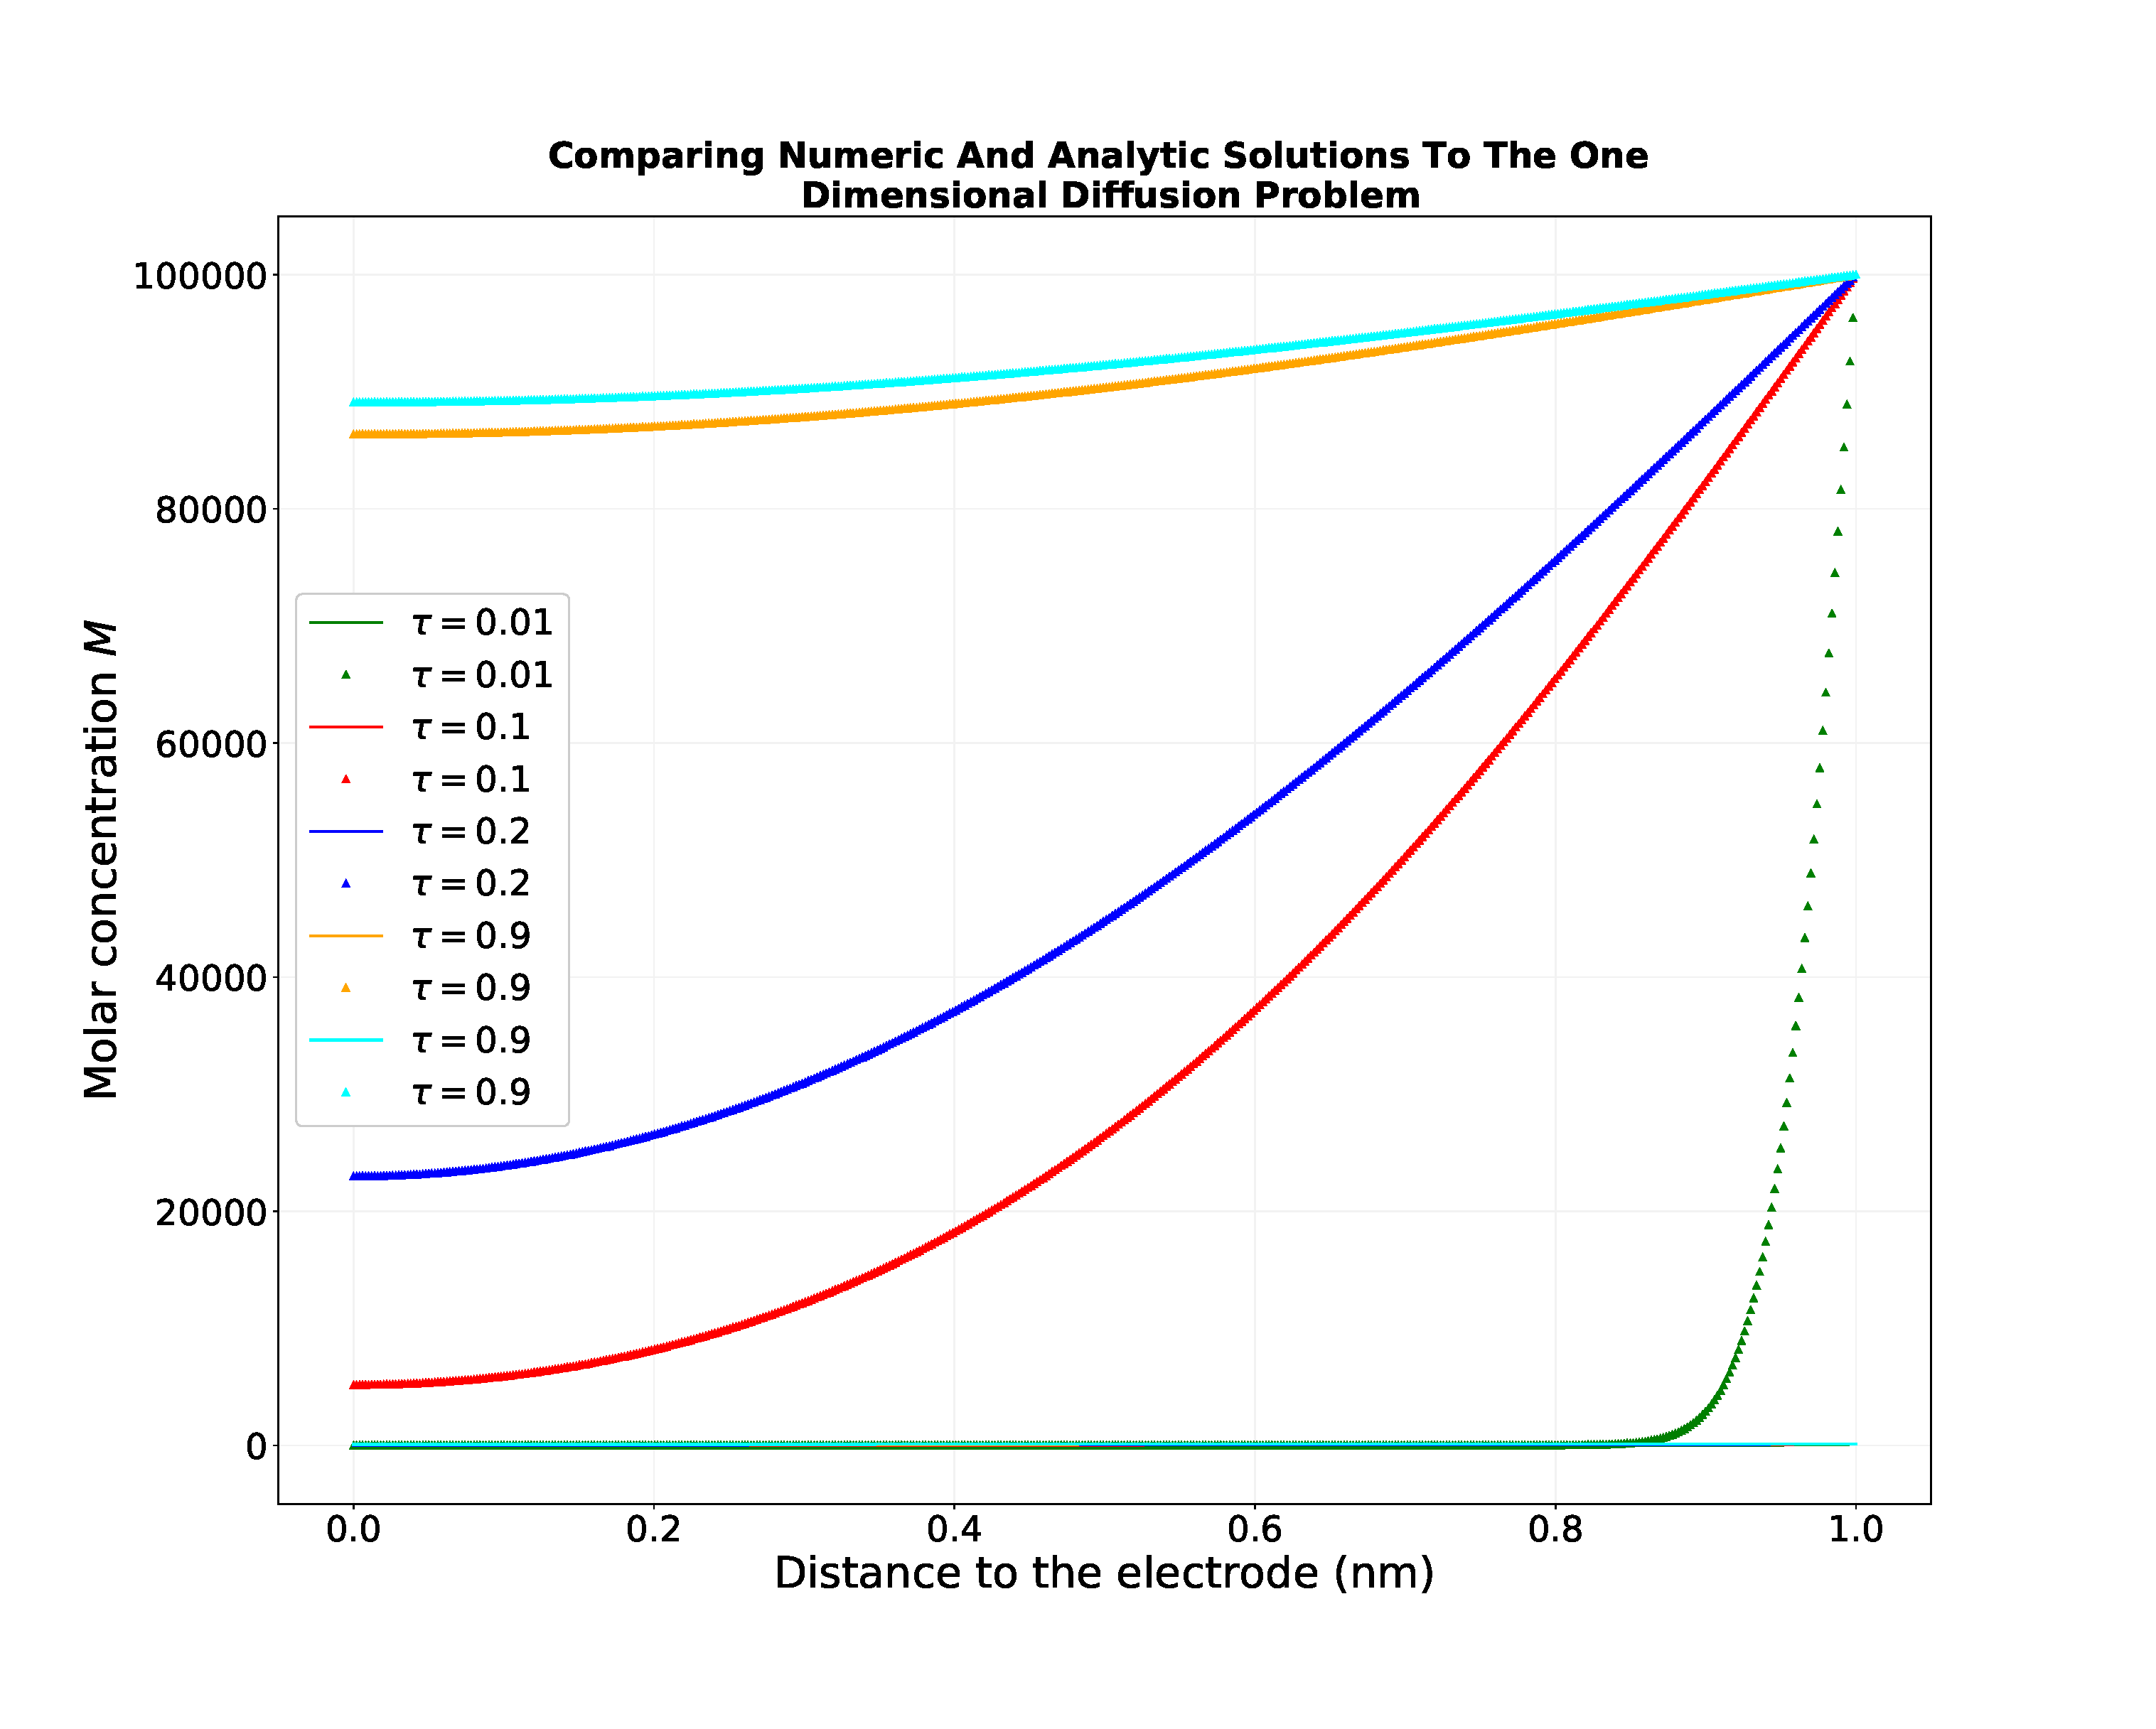
\includegraphics[width=\textwidth]{concentration-diffusiononly-comparison}
\caption{}
\label{fig:diffusion-comparison}
\end{figure}


